\paper{2015}

\question
\begin{parts}
    \part[6]
    Describe when a non-terminal in a grammar
    is called left-recursive,
    when it is called nullable,
    and when it is called useless.
    Provide a short example for each of them.

    \part
    \begin{subparts}
        \subpart[6]
        Demonstrate with a simple example and
        using diagrams that the following grammar
        is ambiguous.
        \[
            E \to E + E \mid E - E \mid (E) \mid \bm{\text{id}}.
        \]

        \subpart[3]
        Rewrite this grammar by applying left factoring to it.
        Does the new grammar become unambiguous?
    \end{subparts}
    
    \part[3]
    In the following grammar, elimate the left
    recursion to obtain an equivalent grammar.
    \begin{align*}
        A &\to Ax \mid Ay \mid Bxy \mid zx \\
        B &\to yB \mid yz
    \end{align*}

    \part[7]
    Lex is a software tool that automatically generates
    a lexical analyser, given a set of patterns
    (regular expressions) with some specific order.
    In particular, Lex simulates an NFA from the given
    patterns.
    It scans the input string until it finds the longest
    prefix of the input that matches one of the given 
    patterns.
    If this longest prefix matches more than one patern,
    then Lex chooses among them the pattern that is first
    in the order.

    Let the three patterns in the picture below be given 
    to Lex (in this order).
    Assuming that the input string is $abbca$,
    find the matching pattern of Lex and the longest
    returned prefix.
    Show all intermediate steps of your computation.

    \begin{center}
        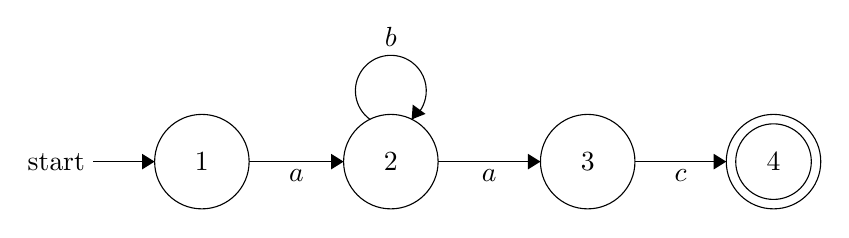
\begin{tikzpicture}[scale=0.2]
            \tikzstyle{every node}+=[inner sep=0pt]
            \draw [black] (14.6,-27.8) circle (3);
            \draw (14.6,-27.8) node {$1$};
            \draw [black] (26.6,-27.8) circle (3);
            \draw (26.6,-27.8) node {$2$};
            \draw [black] (39.1,-27.8) circle (3);
            \draw (39.1,-27.8) node {$3$};
            \draw [black] (50.9,-27.8) circle (3);
            \draw (50.9,-27.8) node {$4$};
            \draw [black] (50.9,-27.8) circle (2.4);
            \draw [black] (7.7,-27.8) -- (11.6,-27.8);
            \draw (7.2,-27.8) node [left] {start};
            \fill [black] (11.6,-27.8) -- (10.8,-27.3) -- (10.8,-28.3);
            \draw [black] (17.6,-27.8) -- (23.6,-27.8);
            \fill [black] (23.6,-27.8) -- (22.8,-27.3) -- (22.8,-28.3);
            \draw (20.6,-28.3) node [below] {$a$};
            \draw [black] (25.277,-25.12) arc (234:-54:2.25);
            \draw (26.6,-20.55) node [above] {$b$};
            \fill [black] (27.92,-25.12) -- (28.8,-24.77) -- (27.99,-24.18);
            \draw [black] (29.6,-27.8) -- (36.1,-27.8);
            \fill [black] (36.1,-27.8) -- (35.3,-27.3) -- (35.3,-28.3);
            \draw (32.85,-28.3) node [below] {$a$};
            \draw [black] (42.1,-27.8) -- (47.9,-27.8);
            \fill [black] (47.9,-27.8) -- (47.1,-27.3) -- (47.1,-28.3);
            \draw (45,-28.3) node [below] {$c$};
        \end{tikzpicture}
    \end{center}
    \begin{center}
        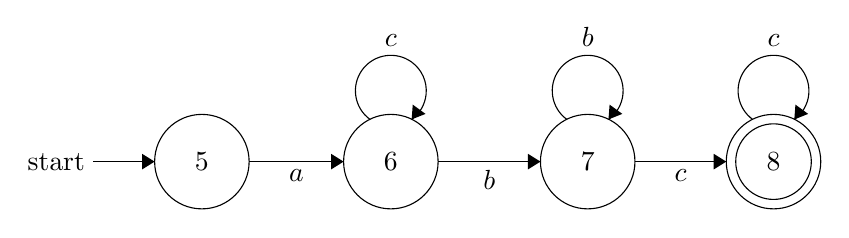
\begin{tikzpicture}[scale=0.2]
            \tikzstyle{every node}+=[inner sep=0pt]
            \draw [black] (14.6,-27.8) circle (3);
            \draw (14.6,-27.8) node {$5$};
            \draw [black] (26.6,-27.8) circle (3);
            \draw (26.6,-27.8) node {$6$};
            \draw [black] (39.1,-27.8) circle (3);
            \draw (39.1,-27.8) node {$7$};
            \draw [black] (50.9,-27.8) circle (3);
            \draw (50.9,-27.8) node {$8$};
            \draw [black] (50.9,-27.8) circle (2.4);
            \draw [black] (7.7,-27.8) -- (11.6,-27.8);
            \draw (7.2,-27.8) node [left] {start};
            \fill [black] (11.6,-27.8) -- (10.8,-27.3) -- (10.8,-28.3);
            \draw [black] (17.6,-27.8) -- (23.6,-27.8);
            \fill [black] (23.6,-27.8) -- (22.8,-27.3) -- (22.8,-28.3);
            \draw (20.6,-28.3) node [below] {$a$};
            \draw [black] (25.277,-25.12) arc (234:-54:2.25);
            \draw (26.6,-20.55) node [above] {$c$};
            \fill [black] (27.92,-25.12) -- (28.8,-24.77) -- (27.99,-24.18);
            \draw [black] (29.6,-27.8) -- (36.1,-27.8);
            \fill [black] (36.1,-27.8) -- (35.3,-27.3) -- (35.3,-28.3);
            \draw (32.85,-28.3) node [below] {$b$};
            \draw [black] (42.1,-27.8) -- (47.9,-27.8);
            \fill [black] (47.9,-27.8) -- (47.1,-27.3) -- (47.1,-28.3);
            \draw (45,-28.3) node [below] {$c$};
            \draw [black] (37.777,-25.12) arc (234:-54:2.25);
            \draw (39.1,-20.55) node [above] {$b$};
            \fill [black] (40.42,-25.12) -- (41.3,-24.77) -- (40.49,-24.18);
            \draw [black] (49.577,-25.12) arc (234:-54:2.25);
            \draw (50.9,-20.55) node [above] {$c$};
            \fill [black] (52.22,-25.12) -- (53.1,-24.77) -- (52.29,-24.18);
        \end{tikzpicture}
    \end{center}
        \begin{center}
        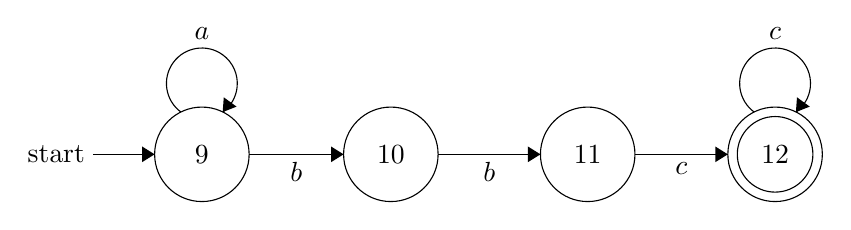
\begin{tikzpicture}[scale=0.2]
            \tikzstyle{every node}+=[inner sep=0pt]
            \draw [black] (14.6,-27.8) circle (3);
            \draw (14.6,-27.8) node {$9$};
            \draw [black] (26.6,-27.8) circle (3);
            \draw (26.6,-27.8) node {$10$};
            \draw [black] (39.1,-27.8) circle (3);
            \draw (39.1,-27.8) node {$11$};
            \draw [black] (51,-27.8) circle (3);
            \draw (51,-27.8) node {$12$};
            \draw [black] (51,-27.8) circle (2.4);
            \draw [black] (7.7,-27.8) -- (11.6,-27.8);
            \draw (7.2,-27.8) node [left] {start};
            \fill [black] (11.6,-27.8) -- (10.8,-27.3) -- (10.8,-28.3);
            \draw [black] (17.6,-27.8) -- (23.6,-27.8);
            \fill [black] (23.6,-27.8) -- (22.8,-27.3) -- (22.8,-28.3);
            \draw (20.6,-28.3) node [below] {$b$};
            \draw [black] (29.6,-27.8) -- (36.1,-27.8);
            \fill [black] (36.1,-27.8) -- (35.3,-27.3) -- (35.3,-28.3);
            \draw (32.85,-28.3) node [below] {$b$};
            \draw [black] (42.1,-27.8) -- (48,-27.8);
            \fill [black] (48,-27.8) -- (47.2,-27.3) -- (47.2,-28.3);
            \draw (45.05,-28.3) node [below] {$c$};
            \draw [black] (49.677,-25.12) arc (234:-54:2.25);
            \draw (51,-20.55) node [above] {$c$};
            \fill [black] (52.32,-25.12) -- (53.2,-24.77) -- (52.39,-24.18);
            \draw [black] (13.277,-25.12) arc (234:-54:2.25);
            \draw (14.6,-20.55) node [above] {$a$};
            \fill [black] (15.92,-25.12) -- (16.8,-24.77) -- (15.99,-24.18);
        \end{tikzpicture}
    \end{center}
\end{parts}

\question
\begin{parts}
    \part[4]
    Briefly describe what the symbol table is in a compiler
    and how it is being used in the analysis part of the
    compiler.

    \part
    \begin{subparts}
        \subpart[3]
        When do we call a Syntax Directed Definition (SDD)
        S-attributed and when do we call it L-attributed?

        \subpart[4]
        Explain why there always exists an evaluation order
        of the attributes in an S-attributed SSD and in an
        L-attributed SSD.
    \end{subparts}

    \part[6]
    Using the following simple Syntax Directed Definition (SDD),
    construct the annotated parse tree for the computation $3*5$.
    \begin{center}
        \begin{tabular}{cll}
            \toprule
            & Production & Semantic rules \\
            \midrule
            1) & $T \to FT'$               & $T'.inh = F.val$ \\
               &                           & $T.val = T'.syn$ \\
            2) & $T' \to *FT_1'$           & $T'_1.inh=T'.inh \cdot F.val$ \\
               &                           & $T'.syn = T_1'.syn$ \\
            3) & $T' \to \varepsilon$      & $T'.syn = T'.inh$ \\
            4) & $F \to \bm{\text{digit}}$ & $F.val = \bm{\text{digit}}.lexval$ \\
            \bottomrule
        \end{tabular}
    \end{center}

    \part[8]
    Construct the leftmost derivation and the rightmost
    derivation of the string $z*(x+y)$ in the following
    grammar (the starting symbol is $S$):
    \begin{align*}
        S &\to S + A \\
        S &\to A \\
        A &\to A * B \\
        A &\to B \\
        B &\to (S) \\
        B &\to a \\
        B &\to b \\
        B &\to c \\
    \end{align*}
\end{parts}
